% =====================================================================
% rankflips.tex: replaces \subsection{The blindness on real generators}
% (\label{app:rankflips}) in sec/X_appendix.tex, from that \subsection line
% through the end of the fig:rankflips float (\label{fig:rankflips} ...
% \end{figure*}). The fig:samples float that follows it in the file is NOT part
% of this replacement; leave it where it is.
% Labels defined here: app:rankflips, tab:rankflips, fig:rankflips (kept),
% app:functional, tab:functional (new).
% Sources: outputs/run_20261108_205428_stats_fixes/rankflips_exact.json (pairs,
% rho), outputs/run_20261109_152704_rankflips_functional_rebase/results.json
% (functional split on the 40 pairs, 34 decisions under the exact test, worked
% examples), outputs/run_20261108_204723_functional_groundtruth/results.json (FD),
% outputs/run_20261106_193513_render_blind_rank_flips/results.md (hidden blocks,
% ceiling, hollowed outputs).
% =====================================================================
\subsection{The blindness on real generators}
\label{app:rankflips}

The probes of the main text alter real builds. This section asks whether the same blindness
changes conclusions about generators. We pool every house generator scored against the
$399$-build validation reference at the protocol's $n$ under the current renderer: $22$
autoregressive voxel models (scale, temperature, best-of-$k$, rejection fine-tuning,
tokenizer and schedule variants), $10$ facade generators, which emit the six face images of
a build and lift them into the voxel grid, $5$ LLM program generators, the two clean 3D-BPE
models of the leaderboard and BrickNet \citep{kulits2026bricknet}, $40$ in all, $35$ of them
at $n{=}256$ and the LLM arms at $n{=}128$ to $133$. Both metrics are recomputed from the
per-build features of every arm, matched to its card by hash (\mvkid{} to $3\times10^{-6}$).
Every pair is tested with the exact label-permutation test of Sec.~\ref{app:significance}
against the fixed reference, $20{,}000$ permutations, Holm-corrected over all $780$ pairs per
metric. The test stays exact at unequal sizes, and the $35$ arms at $n{=}256$ are also
reported alone. The interval on $\rho$ half-samples every arm and the reference jointly.

\begin{table}[h]
\centering
\small
\setlength{\tabcolsep}{4pt}
\caption{\textbf{Agreement of the two rankings over real generators.} Spearman correlation
of the \mvkid{} and \vkid{} orderings with a half-sampling $95\%$ interval. Pairs: separated
by both metrics under the exact permutation test after Holm correction over all $780$, and
the subset the two metrics order oppositely.}
\label{tab:rankflips}
\resizebox{\linewidth}{!}{%
\begin{tabular}{lrccc}
\toprule
generators & $k$ & $\rho$ & both sep. & opposite \\
\midrule
all & $40$ & $0.50$ \scriptsize{$[0.37, 0.58]$} & $308$ & $\mathbf{40}$ \\
at $n{=}256$ & $35$ & $0.60$ \scriptsize{$[0.46, 0.67]$} & $255$ & $24$ \\
autoregressive voxel & $24$ & $0.37$ \scriptsize{$[0.16, 0.51]$} & $58$ & $7$ \\
facade & $10$ & $0.99$ \scriptsize{$[0.88, 1.00]$} & $32$ & $0$ \\
\bottomrule
\end{tabular}}
\end{table}

\paragraph{Where the rankings part.} The interval of Table~\ref{tab:rankflips} reflects
sampling of builds. Resampling the generators themselves widens it to $[0.20, 0.72]$, and a
cluster bootstrap over the five families to $[0.02, 0.91]$: the correlation is a property of
this pool's family mix. Without the facade family it is $0.28$; without the voxel family,
$0.72$. In $22$ of the $40$ reversed pairs the render metric prefers a facade generator.
Facade generators emit shells: a median $0.5\%$ of their blocks have no face on exterior air,
against $15.6\%$ for held-out houses and $12.5\%$ for the voxel models, and moving from the
\mvkid{} to the \vkid{} ranking costs the family $7.7$ places on average. Across all $40$
generators, however, the shift between the two rankings correlates with the share of hidden
blocks only at $\rho{=}-0.26$ ($p{=}0.10$), so hidden mass alone does not explain the
reordering. The pair of Fig.~\ref{fig:rankflips} is tied under \mvkid{}, $3.1$ noise floors
apart (Holm $p{=}1$), and $292.9$ floors apart under \vkid{} (Holm $p{=}0.039$, the smallest
value $20{,}000$ permutations can reach over $780$ pairs); with the roof removed, the facade
builds are walls around an empty floor. Next to the same voxel model, a best-of-four facade
generator is preferred by \mvkid{} by $55.1$ floors and rejected by \vkid{} by $209.5$, both
at the same Holm floor.

\paragraph{The ceiling of a shell generator.} Reducing each held-out house to the cells its
six faces show gives the output of a perfect facade generator. It sits $8.1$ noise floors
from real data under \mvkid{}, ahead of every trained generator by more than $90$ floors,
and at $+310.6$ under \vkid{}, $19$th of $41$. Applied to generator output, \hollow{}
deletes the blocks no camera sees from our best voxel model, $15\%$ of its mass, and moves
it from $5$th to $29$th of $41$ under \vkid{} ($+147.5$ floors). On the same $128$ builds,
rendered and scored together with their hollowed copies, \mvkid{} moves $+0.15$ noise floors
and \vkid{} $+117.1$; for the 3D-BPE model the two read $+0.18$ and $+139.2$. The converse
holds as well: a voxel model sampled at temperature $0.7$ is over-solid, $24\%$ hidden
blocks, and hollowing its output moves it $24.7$ floors \emph{closer} to real data under
\vkid{}. \vkid{} therefore sees what is deleted from a generator's interior; whether what it
sees is damage is a separate question, which Sec.~\ref{app:functional} answers.

\paragraph{Design decisions.} We list $34$ decisions taken while building these generators,
each a pair of arms that differ in one choice (temperature, best-of-$k$, rejection
fine-tuning, scale, D4 augmentation, tokenizer, schedule, LLM loop), and test each with the
same exact permutation test, Holm-corrected over the $34$. The two metrics agree on $6$ and
never disagree in sign when both are significant; $13$ are significant under neither. On
$15$ the verdict depends on the pillar: $14$ are significant under \mvkid{} alone, among them
D4 augmentation of the 20M facade model ($-52.4$ floors under \mvkid{}, $+16.9$ under
\vkid{}), and $1$ under \vkid{} alone, replacing voxels with 3D-BPE pieces ($+162.6$ floors
worse under \vkid{}, $+21.5$ under \mvkid{}). Most decisions that change a score change
what the exterior shows; local geometry moves beyond noise in $7$ of the $34$.

\paragraph{Scope.} The $40$ generators come from one project. \vkid{} is a distribution
distance on local geometry, not a counter of hidden blocks: the LLM program arms are also
near-shells and move up, not down, under \vkid{}, and the best facade generator has the
lowest \vkid{} of the pool, below its own ceiling, because sampling at temperature $0.7$
narrows its size and shape distribution toward the reference mode. Under the
$80$-dimensional descriptor of the current cards, $29$ of the $308$ both-separated pairs
reverse and the correlation rises to $0.65$ $[0.54, 0.71]$; every statement above holds.

\begin{figure*}[t]
\centering
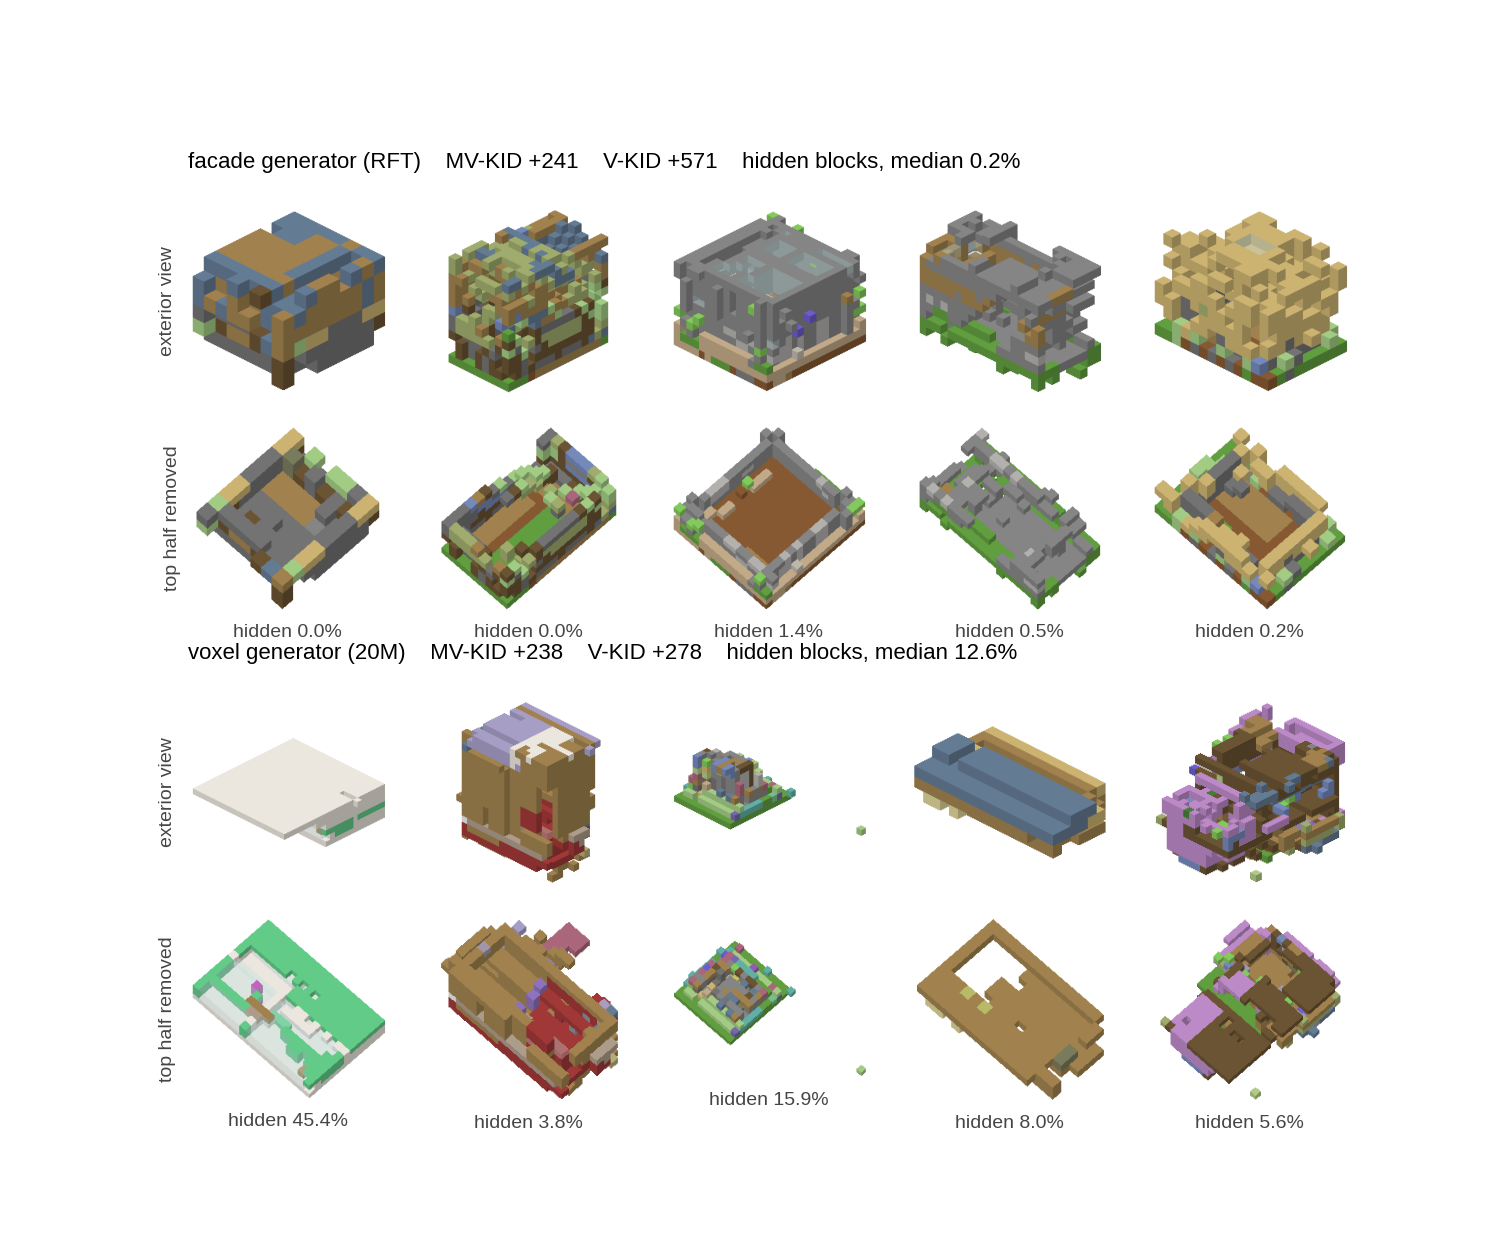
\includegraphics[width=0.8\linewidth]{figures/rankflips_samples}
\caption{\textbf{Tied under \mvkid{}, $293$ floors apart under \vkid{}.} The first five
builds of each arm that pass the memorization gate, generated output only. Top of each block:
the exterior corner view of the protocol; bottom: the same build with its upper half
removed. The facade generator's builds are walls around an empty floor, a median $0.2\%$ of
blocks hidden from every exterior ray; the voxel model's hold partitions and fill, $12.6\%$
($15.6\%$ for held-out houses).}
\label{fig:rankflips}
\end{figure*}

\subsection{Detection is not ranking: a functional ground truth}
\label{app:functional}

The probes establish that \vkid{} detects a change to a real interior that \mvkid{} cannot
see. On the $40$ reversed pairs the question is different: which ranking orders generators
by how usable their interiors are. We answer it with a test that reads neither metric's
features.

\paragraph{A walk-through test.} Every build is set on flat ground and entered by the player
of the traversability probe, a body two blocks tall that steps up one block, falls, climbs
ladders and opens doors. Five measures follow: whether the player reaches any interior
standing cell (\emph{enterable}); how many interior standing cells it reaches (\emph{floor});
how many rooms it reaches, a room being a component of interior air holding at least six
standing cells, with doorways closed so that a doorway separates two rooms; whether at least
half of the plan is roofed by a block with two free cells beneath it; and the share of blocks
in the largest 6-connected component. Held-out houses average $0.94$, $80$ cells, $1.36$
rooms, $0.81$ and $0.98$. \vkid{} has no reachability, door semantics, room labelling, plan
shelter or component analysis; a cross-validated ridge regression on its $77$ features
explains $R^2 = 0.29$ to $0.62$ of the per-build measures. The functional distance FD of an
arm is the mean over the five measures of the Wasserstein-1 distance to the validation
reference, each in units of the real between-build spread, with $1{,}000$ bootstrap
replicates that share one reference resample. Three variants check the construction: units
of real-versus-real sampling distance at $n{=}256$, a cubic-kernel KID on the standardized
measures, and an occupancy-only version without door semantics.

\paragraph{The test sees interiors.} Held-out real data ranks first of $41$ under all four
variants, at FD $0.09$ $[0.08, 0.19]$ against $0.52$ for the best generator. \solidify{}
reaches $1.21$, cutting the enterable share from $0.94$ to $0.20$, and \hollow{} $0.60$:
the walk-through detects the two probes \mvkid{} cannot, so its verdict on generators is not
a second exterior observer.

\paragraph{On generators it follows the render ranking.} Over the $40$ generators, FD
correlates with \mvkid{} at Spearman $0.67$ $[0.41, 0.82]$ and with \vkid{} at $0.16$
$[-0.20, 0.45]$, with intervals that resample generators and FD replicates jointly. The
maximum of the two, which \blockscore{} reads, correlates at $0.17$ $[-0.18, 0.45]$, because
geometry is the worse pillar for $37$ of the $40$. On the $40$ reversed pairs, every FD
difference is significant, and the walk-through sides with \mvkid{} in $33$ and with \vkid{}
in $7$ ($18\%$, Clopper--Pearson $[7, 33]$). The facade family does not produce this. On the
$18$ pairs without a facade generator it sides with \vkid{} in none ($[0, 19]\%$); on the
$22$ facade pairs it does so in $7$, five of them BrickNet preferred over a facade generator,
and BrickNet's builds are almost never enterable ($0.8\%$). The variants agree ($2$, $9$ and
$8$ of $40$ for the noise-unit, KID and occupancy-only distances; none of the $18$
non-facade pairs under the occupancy-only one), and leaving out any one generator keeps the
share between $6\%$ and $24\%$. Taken one measure at a time, enterability, reached floor and
reached rooms side with \vkid{} on none of the $40$.

\paragraph{Why.} The autoregressive voxel generators do not emit shells; they clutter their
interiors. A median $22\%$ of their builds can be entered, against $94\%$ of held-out houses,
with a median $3.4$ reachable floor cells against $80$. Their walls, block patterns and
sealed air have the local statistics of real houses, and \vkid{} scores those statistics.
Deleting the hidden blocks of the best voxel model moves it $147.5$ \vkid{} floors away from
real data and $0.41$ functional units toward it ($1.32$ to $0.90$), and the one design
decision \vkid{} alone flags, 3D-BPE pieces over voxels, is one the walk-through prefers
($1.34$ against $1.67$). Detection of interior change is not ranking of interior function.
The probes hold, since \solidify{} and \hollow{} are functional damage on real houses that
renders cannot see. On current generators, though, the dominant interior failure co-varies
with defects the render tier sees, and a local volumetric descriptor reads it as realism. A
leaderboard that ranks by interior function needs a functional pillar beside both tiers.

\begin{table}[h]
\centering
\small
\setlength{\tabcolsep}{3pt}
\caption{\textbf{Functional ground truth.} Top: functional distance to real (FD, $95\%$
bootstrap interval) and enterable share. Bottom: on the $40$ pairs the two metrics order
oppositely, how often the walk-through agrees with each, and its Spearman correlation with
each ranking over the $40$ generators.}
\label{tab:functional}
\resizebox{\linewidth}{!}{%
\begin{tabular}{lcc}
\toprule
arm & FD & enterable \\
\midrule
held-out real & $0.09$ \scriptsize{$[0.08, 0.19]$} & $0.95$ \\
\solidify{} & $1.21$ \scriptsize{$[1.11, 1.32]$} & $0.20$ \\
\hollow{} & $0.60$ \scriptsize{$[0.52, 0.73]$} & $0.95$ \\
best generator (LLM program) & $0.52$ \scriptsize{$[0.43, 0.65]$} & $0.68$ \\
best voxel model under \vkid{} & $1.32$ \scriptsize{$[1.20, 1.43]$} & $0.28$ \\
\quad same, hidden blocks deleted & $0.90$ \scriptsize{$[0.78, 1.04]$} & $0.59$ \\
\midrule
 & with \mvkid{} & with \vkid{} \\
reversed pairs, all $40$ & $33$ & $7$ \\
reversed pairs, $18$ without a facade arm & $18$ & $0$ \\
reversed pairs, $22$ with a facade arm & $15$ & $7$ \\
Spearman over $40$ generators & $0.67$ \scriptsize{$[0.41, 0.82]$} & $0.16$ \scriptsize{$[-0.20, 0.45]$} \\
\bottomrule
\end{tabular}}
\end{table}
